\subsection{Demostración}

\underline{Aclaración:} Al ser un árbol, sabemos que hay una única forma de llegar de un nodo A a uno B (pasando una vez por cada arista) por lo tanto si B tiene k ramas adyacentes, en el momento que llego a B (recorriendo siempre hacia un adyacente) sólo una de esas ramas puede estar explorada (en las demás aún no pude alcanzar ningún nodo). Si hubiese ya alcanzado algun nodo en una de las otras ramas, entonces si sigo recorriendo esa rama lo podría alcanzar nuevamente e ir desde allí hacia el nodo donde comencé generando un ciclo simple, lo cual es absurdo porque en un árbol no tengo ciclos simples.
\begin{center}
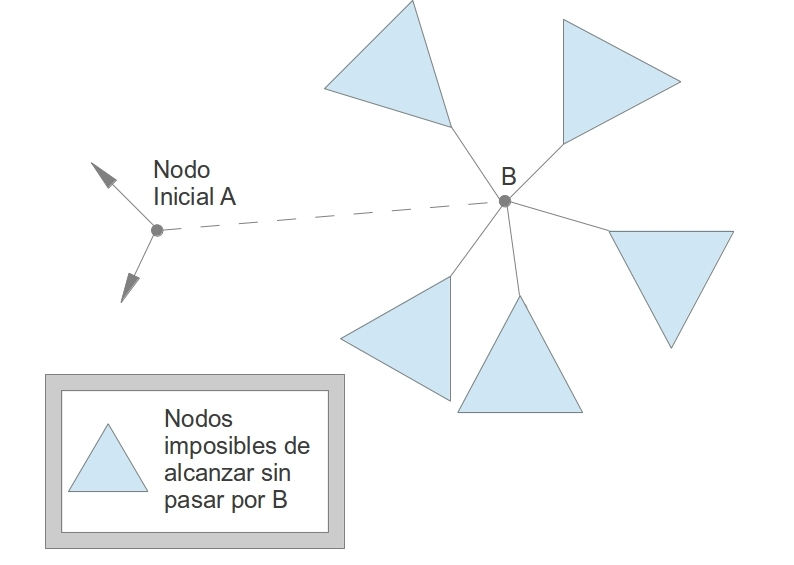
\includegraphics[scale=0.5]{ej2/2/graficos/imagen02.jpg} 
\end{center}
Dado un árbol de n nodos, elijo un nodo P cuyas dos ramas más largas conforman un camino de longitud máxima del árbol (r1 tiene una longitud de h y r2 una longitud de i con i $\leq$ h, i puede ser cero), además estas ramas difieren en a lo sumo una arista de longitud (entonces i = h-1 o i = h).

De P se desprenden k aristas (k < n) y aquellas que no son r1 y r2 sabemos que tienen una longitud máxima menor o igual a r2. Entonces elegir a P como master me resuelve el problema en h pasos (h $\geq$ i $\geq$ resto de ramas) además h + i = longitud de camino máximo.
\begin{center}
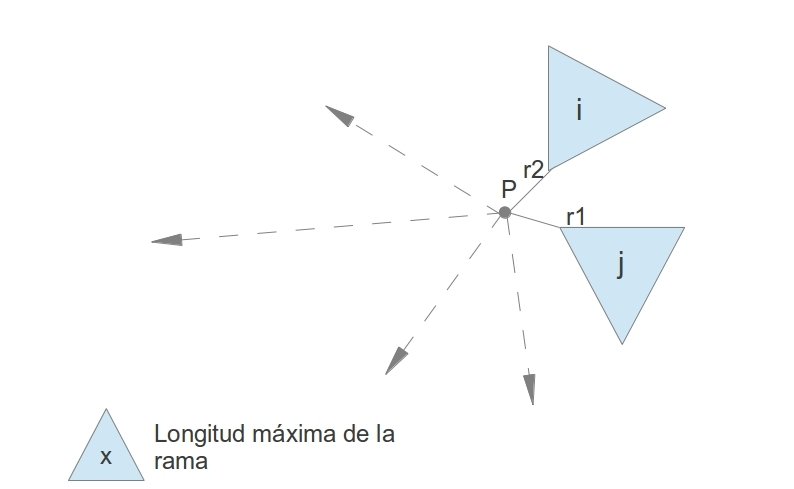
\includegraphics[scale=0.4]{ej2/2/graficos/imagen03.jpg} 
\end{center}
Ahora supongo que existe otro nodo P' que me resuelve el problema en menos pasos, entonces llegar al nodo P me va a llevar cierta cantidad de pasos j, con j $\geq$ 1, y en el momento de llegar a P al menos una de las dos ramas (r1 o r2) no puede haber sido atravesada en absoluto, es decir en alguna de las ramas ningún nodo fue alcanzado todavía (ver Aclaración del comienzo). 

Por lo tanto al menos voy a necesitar recorrer alguna de ellas para completar el recorrido por todos los nodos del árbol, suponiendo que estoy en mi mejor caso y que me queda recorrer la rama r2 que tiene longitud menor o igual a r1, le sumo los pasos que me costó llegar a P nos queda: como j $\geq$ 1 y long(r2)=i $\Rightarrow$ i + j, además sé que i= h-1 o i=h $\Rightarrow$  h - 1 + j $\geq$ h ó h + j > h
Así la cantidad de pasos no puede ser menor si elijo P', a lo sumo es igual. Por lo tanto P está bien escogido, aunque no sea la única solución.


La implementación encuentra un nodo de un camino máximo y luego haciendo el 'balanceo' llego a un master óptimo.

Lo que tengo que demostrar es que empezando desde un nodo C cualquiera y recorriendo sus adyacentes (sin volver nunca por donde vine) en algún momento entro en un camino máximo y la longitud del mismo la puedo calcular como la suma de las dos ramas más largas del nodo (sin contar la rama por la que vine, y teniendo en cuenta la aclaración).

Tengo dos casos, que el nodo donde arranco no pertenezca a un camino máximo, o que pertenezca.
\begin{itemize}

\item Si no pertenece, en algún momento llego a un nodo M que si pertenece, si sumo las dos ramas más largas de M voy a tener la longitud del camino máximo. Puedo afirmar ésto porque la rama por la cual llego a M, no puede tener una longitud mayor a ninguna de sus dos ramas más largas, ya que si fuera así el camino máximo tendría que involucrar al nodo anterior por el que ya pasé adyacente a M, pero es falso porque dijimos que M era el primer nodo que alcanzamos que pertenecía a un camino máximo.

\item Si arranco en un nodo perteneciente a un camino máximo, la suma de sus ramas más largas es igual a la longitud de dicho camino. Esto es verdad siempre, si r1 y r2 son mis ramas más largas, longmax(r1)$\geq$ longmax(r2)$\geq$ otras ramas, el camino máximo que pasa por este nodo es igual a longmax(r1) + longmax(r2).
\end{itemize}

Ya vimos que requisitos cumple un master óptimo, y luego que la implementación encuentra un nodo de un camino máximo, falta un último detalle y es el 'balanceo'.
El nodo que encontramos pertenece al camino máximo, y moviendome hacia el nodo adyacente con la rama más larga (siempre me mantengo en el camino máximo) en algún momento tengo que encontrar un nodo cuyas dos ramas más largas sean iguales o difieran en una arista de longitud. La forma en que se implementa se puede ver en el pseudocódigo del algoritmo EncontrarMaster, o en el código fuente.

